\documentclass[11pt]{article}
\usepackage{euscript}

\usepackage{amsmath}
\usepackage{amsthm}
\usepackage{amssymb}
\usepackage{epsfig}
\usepackage{xspace}
\usepackage{color}
\usepackage{url}
\usepackage{subfig}
\usepackage{float}
\usepackage{array}
\graphicspath{ {images/} }
%%%%%%%  For drawing trees  %%%%%%%%%
\usepackage{tikz}
\usetikzlibrary{calc, shapes, backgrounds}

%%%%%%%%%%%%%%%%%%%%%%%%%%%%%%%%%
\setlength{\textheight}{9in}
\setlength{\topmargin}{-0.600in}
\setlength{\headheight}{0.2in}
\setlength{\headsep}{0.250in}
\setlength{\footskip}{0.5in}
\flushbottom
\setlength{\textwidth}{6.5in}
\setlength{\oddsidemargin}{0in}
\setlength{\evensidemargin}{0in}
\setlength{\columnsep}{2pc}
\setlength{\parindent}{1em}
%%%%%%%%%%%%%%%%%%%%%%%%%%%%%%%%%


\newcommand{\eps}{\varepsilon}

\renewcommand{\c}[1]{\ensuremath{\EuScript{#1}}}
\renewcommand{\b}[1]{\ensuremath{\mathbb{#1}}}
\newcommand{\s}[1]{\textsf{#1}}
\newcommand{\tb}[1]{\textbf{#1}}

\newcommand{\E}{\textbf{\textsf{E}}}
\renewcommand{\Pr}{\textbf{\textsf{Pr}}}
\newcommand*{\escape}[1]{\texttt{\textbackslash#1}}


\title{\textbf{\underline{Asmt 3: Clustering}}}
%\footnote{\s{CS 6140  Data Mining; \;\; Spring 2015 \hfill
%Instructor: Jeff M. Phillips, University of Utah}
%}

\author{Anirudh Narasimhamurthy(u0941400)}

\begin{document}
\maketitle

\section{Hierarchical Clustering}

\begin{itemize}
	
	
	\item[] In this part of the assignment we are working on the different variants of hierarchical clutsering.For all the sub-sections below, I ran my clustering algorithms until I was left with \emph{k} = 4 clusters. 
	
	\item[] \underline{\textbf{Single-Link Hierarchical clustering}}
	
	In single-link hierarchical clustering, the distance between two clusters $S_1$ and $S_2$ is measured as follows:
	\begin{center}
		$d(S_1,S_2)= \underset{(s_1,s_2) \in S_1 \times S_2}{\min} || s_1 -s_2||_2$
	\end{center}
	
	In our given problem we start with 20 clusters. At every step we find the two clusters which are closest to each other by taking the minimum of the shortest link distance measured using the expresssion above and then merge the two clusters into one. I repeat this process until I am left with k=4 clusters.\\
	
	The results of running the single-link clustering algorithm on data set C1.txt is tabulated below. I have provided the results for each of the four clusters in terms of both their indexes and exact co-ordinates values :
	
	\textbf{Indexes:}
	
	\begin{table}[h]
		\centering
		\begin{tabular}{|c|c|}
			\hline
			\textbf{Set}  & \textbf{Indexes of the points/clusters included in the set} \\
			\hline
			\textbf{Set 1}  & 17\\
			\hline
			\textbf{Set 2} & 2, 9, 12, 15, 16   \\
			\hline
			\textbf{Set 3} &  3, 5, 11, 18, 20    \\
			\hline
			\textbf{Set 4}  & 1, 6, 8, 13, 14, 19, 7, 10   \\
			\hline
		\end{tabular}
		\caption{Single-link Hierarchical clustering }
		\label{t2}
	\end{table}
	
	
	\textbf{ Co-ordinates}
	
			\begin{itemize}
			 \item[]	\textbf{Set 1:}  \{(0.03184434259, 0.7754395581)\}\\
			
			\item[] \textbf{Set 2 :}  \{(0.3642643827, 0.7926049686), (0.3435737692, 0.8225675015), (0.3857244557, 0.7378034552), (0.4139357784, 0.667019538), (0.5329886024, 0.8206248404)\}   \\
	
		 \item[] \textbf{Set 3 :}  \{(0.09266339524, 0.2884581315), (0.1078682625, 0.3174124153), (0.005391164973, 0.2468978009), (0.004697542323, 0.2269133612), (0.1146112415, 0.1433136304), (0.1750281409, 0.5407512275)\}
	
		\item[] \textbf{Set 4 :}  \{ (0.965549653, 0.8590997552), (0.8357557743, 0.818109871), (0.7771284335, 0.660070475), (0.7082581828, 0.4803427579), (0.761212097, 0.4083187031), (0.4860673038, 0.3603060044), (0.7412324486, 0.1429641356), (0.7933397, 0.08918497153)\}
	
		\end{itemize}
	
		I also plotted the results which I had obtained to verify if it was performing it correctly and I felt the results were good enough after seeing the points in the scatter plot. The results are shown below:
	
		\begin{figure}[H]%
			\centering
			\subfloat[Single link hierarchical clustering]{{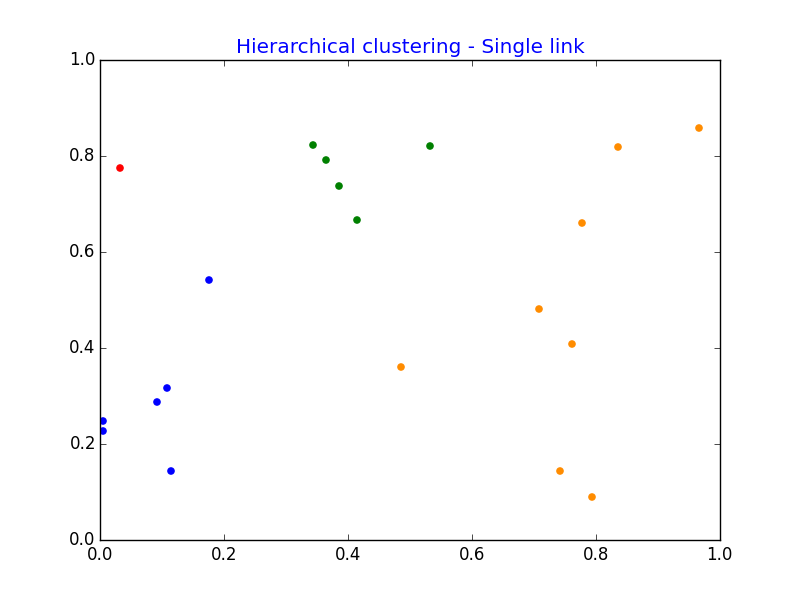
\includegraphics[width=5cm]{Single_link} }}%
		\end{figure}
	
		I have used four different colors to plot/highlight the four different clusters.\\
	
		

	\item[] \underline{\textbf{Complete-Link Hierarchical Clustering}}\\
	
	In complete-link hierarchical clustering, the distance between two clusters $S_1$ and $S_2$ is measured as follows:
	\begin{center}
		$d(S_1,S_2)= \underset{(s_1,s_2) \in S_1 \times S_2}{\max} || s_1 -s_2||_2$
	\end{center}
	
	In our given problem we start with 20 clusters. At every step we find the two clusters which are farthest to each other by taking the minimum of the complete link distance measured using the expresssion above and then merge the two clusters into one. I repeat this process until I am left with k=4 clusters. In other words it is kind of min of max formulation.\\
	
	The results of running the complete-link clustering algorithm on data set C1.txt is tabulated below. I have provided the results for each of the four clusters in terms of both their indexes and exact co-ordinates values :
	
	\textbf{ Co-ordinates}
	
	\begin{itemize}
		\item[]	\textbf{Set 1:}  \{ (0.09266339524, 0.2884581315), (0.1078682625, 0.3174124153), (0.005391164973, 0.2468978009), (0.004697542323, 0.2269133612), (0.1146112415, 0.1433136304)\}\\
		
		\item[] \textbf{Set 2 :}  \{(0.7412324486, 0.1429641356), (0.7933397, 0.08918497153), (0.4860673038, 0.3603060044)\}   \\
		
		\item[] \textbf{Set 3 :}  \{ (0.7082581828, 0.4803427579), (0.761212097, 0.4083187031), (0.7771284335, 0.660070475), (0.965549653, 0.8590997552), (0.8357557743, 0.818109871)\}
		
		\item[] \textbf{Set 4 :}  \{ (0.965549653, 0.8590997552), (0.8357557743, 0.818109871), (0.7771284335, 0.660070475), (0.7082581828, 0.4803427579), (0.761212097, 0.4083187031), (0.4860673038, 0.3603060044), (0.7412324486, 0.1429641356), (0.7933397, 0.08918497153)\}
		
	\end{itemize}
	
	\textbf{Indexes:}
		
		\begin{table}[h]
			\centering
			\begin{tabular}{|c|c|}
				\hline
				\textbf{Set}  & \textbf{Indexes of the points/clusters included in the set} \\
				\hline
				\textbf{Set 1}  & 3, 4, 5, 11, 18\\
				\hline
				\textbf{Set 2} & 7, 8, 10   \\
				\hline
				\textbf{Set 3} &  1, 6, 13, 14, 19   \\
				\hline
				\textbf{Set 4}  & 2, 9, 12, 15, 16, 17, 20   \\
				\hline
			\end{tabular}
			\caption{Complete-link Hierarchical clustering }
			\label{t2}
		\end{table}
		
	
	I also plotted the results which I had obtained to verify if it was performing it correctly and I felt the results were good enough after seeing the points in the scatter plot. The results are shown below:
	
	\begin{figure}[H]%
		\centering
		\subfloat[Complete link hierarchical clustering]{{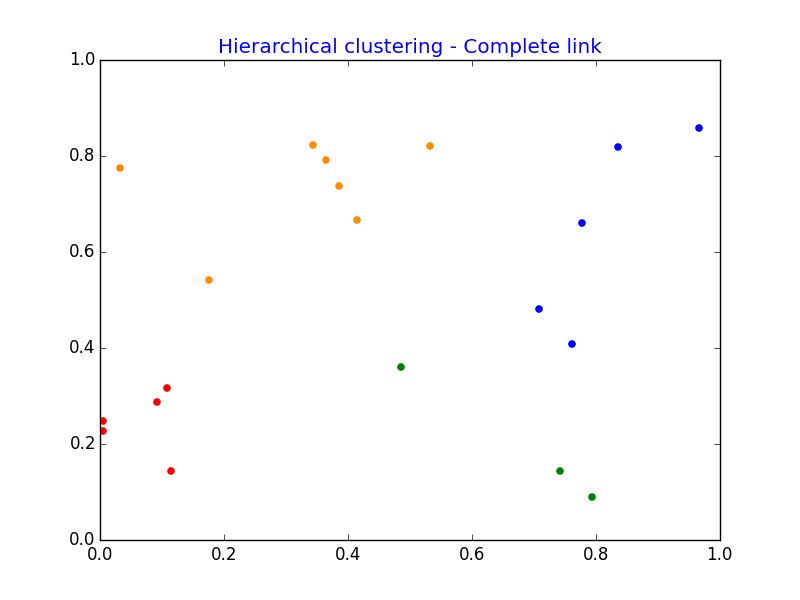
\includegraphics[width=5cm]{Complete_link} }}%
	\end{figure}
	
	I have used four different colors to plot/highlight the four different clusters.
	
	\item[] \underline{\textbf{Mean-Link Hierarchical Clustering}}\\
	
	In mean-link hierarchical clustering, we measure the distances to the means and it is given  as follows:
	\begin{center}
		
		$a_1 = \frac{1}{|S_1|} \sum_{s \in S_1}^{} s $ and \\
		$a_2 =\frac{1}{|S_2|} \sum_{s \in S_2}^{} s $ Then \\
		$d(S_1,S_2)=  || a_1 -a_2||_2$
	\end{center}
	
	In our given problem we start with 20 clusters.At every step we find the mean distances of the clusters. We then merge two  clusters whose mean distances are minimum.I repeat this process until I am left with k=4 clusters.\\
	
	The results of running the mean-link clustering algorithm on data set C1.txt is tabulated below. I have provided the results for each of the four clusters in terms of both their indexes and exact co-ordinates values :
	
	\textbf{ Co-ordinates}
	
	\begin{itemize}
		\item[]	\textbf{Set 1:}  \{  (0.09266339524, 0.2884581315), (0.1078682625, 0.3174124153), (0.005391164973, 0.2468978009), (0.004697542323, 0.2269133612), (0.1146112415, 0.1433136304) \}\\
		
		\item[] \textbf{Set 2 :}  \{ (0.965549653, 0.8590997552), (0.8357557743, 0.818109871), (0.7771284335, 0.660070475)\}   \\
		
		\item[] \textbf{Set 3 :}  \{  (0.7082581828, 0.4803427579), (0.761212097, 0.4083187031), (0.4860673038, 0.3603060044), (0.7412324486, 0.1429641356), (0.7933397, 0.08918497153)\}
		
		\item[] \textbf{Set 4 :}  \{  (0.1750281409, 0.5407512275), (0.03184434259, 0.7754395581), (0.4139357784, 0.667019538), (0.3857244557, 0.7378034552), (0.3642643827, 0.7926049686), (0.3435737692, 0.8225675015), (0.5329886024, 0.8206248404)  \}
		
	\end{itemize}
	
	\textbf{Indexes:}
	
	\begin{table}[h]
		\centering
		\begin{tabular}{|c|c|}
			\hline
			\textbf{Set}  & \textbf{Indexes of the points/clusters included in the set} \\
			\hline
			\textbf{Set 1}  & 3, 4, 5, 11, 18\\
			\hline
			\textbf{Set 2} & 1,13,14   \\
			\hline
			\textbf{Set 3} &  6, 7, 8, 10, 19  \\
			\hline
			\textbf{Set 4}  & 2, 9, 12, 15, 16, 17, 20   \\
			\hline
		\end{tabular}
		\caption{Mean-link Hierarchical clustering }
		\label{t2}
	\end{table}
	
	
	I also plotted the results which I had obtained to verify if it was performing it correctly and I felt the results were good enough after seeing the points in the scatter plot. The results are shown below:
	
	\begin{figure}[H]%
		\centering
		\subfloat[Mean link hierarchical clustering]{{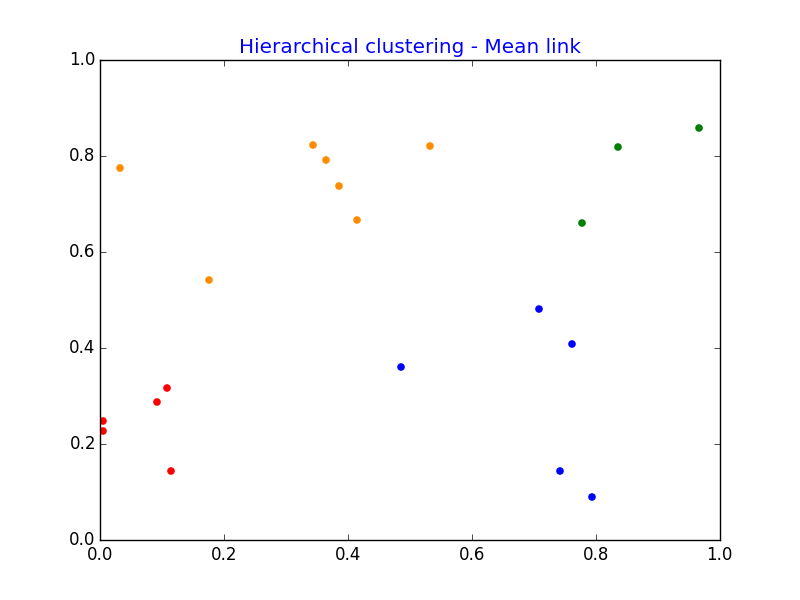
\includegraphics[width=5cm]{Mean_link} }}%
	\end{figure}
	
	On comparing the results provided by all the three clustering algorithms, I felt the result provided by single-link clustering algorithm was very good. And the reasons for it are as follows:
	
	\begin{itemize}
		\item We want the the split or the inter-cluster distance to be as large as possible generally for obtaining a good clustering of data.
		\item We want the width or the intra-cluster distance to be as small as possible generally for obtaining a good clustering of data.
		\item For the given data set the single link clustering algorithm does a very good job on both these fronts. 
		\item The cluster or the point with index 17 could be marginally considered as  an outlier point as it is not nearer to any of the other points. Single link clustering keeps it as a separate cluster in the case of \emph k=4 clusters while both complete-link and mean-link have few other points surrounding the point 17 in a cluster.
	\end{itemize}	
	
	Having said that complete-link and mean-link also did a good enough job of clustering the data and depending upon the data set they might be more beneficial.\\
	
	The variant which was easiest to compute was the \textbf{Single-link}. It was a straight forward min of min operations. Even if the number of data points were to be huge it would still scale well is what I personally feel. Also there are several ways to optimize the process of finding the minimum element and if we were to use iterator tools package available in python we could reduce the combinations of elements which we compare and hence we could optimize the entire process to produce good results in a reasonable amount of time using single link clustering.\\
	
	\textbf{Mean-link hierarchical clustering} on the other hand would definitely be the worst in terms of computation as we are required to calculate the mean of all the points and then compare the distances based on the means. Calculating the means is not a cheaper operation as it requires us to go over all the elements in the data set and re-calculate it again.
	
	
	\end{itemize}




	
\section{Point Assignment Clustering}

\begin{itemize}
	
\item[] \textbf{ Part A}
	
\item[] \underline{\textbf{Gonzalez Algorithm}}

In Gonzalez algorithm for our given problem we start with $c_1$ to be the point with index 1. The Gonzalez algorithm basically then tries to find the next center which is farthest from the current center. And it then finds the third center which is farthest from our first two centers. Since k=3 we are required to stop once we have the three centers.

In this section, all the algorithms are run on the data set C2. txt

After running the Gonzalez algorithm, the centers and the subsets obtained are shown below:


 \textbf{Centers} :  \textbf{\{  (-19.0748, -8.536), (-40.0, 40.0), (29.10710988, -8.527838244)   \}}\\
\textbf{ 3-center cost:  39.6823111475 }\\
\textbf{ 3-means cost:  311124.602477}\\
\pagebreak


The subsets obtained are shown below. I have provided the indexes of the points used in the data set rather than specifying the full co-ordinates as it made the document too cluttered and wasted a lot of pages. I am hoping this should suffice. \\

\underline{\textbf{Subsets}}

\textbf{Indexes of the points which have their center as (-19.0748, -8.536)}

[1, 4, 5, 6, 7, 8, 9, 10, 11, 12, 13, 14, 15, 16, 17, 18, 19, 20, 21, 22, 23, 24, 25, 26, 27, 28, 29, 30, 31, 32, 33, 34, 35, 36, 37, 38, 39, 40, 41, 42, 43, 44, 45, 46, 47, 48, 49, 50, 51, 52, 53, 54, 55, 56, 57, 58, 59, 60, 61, 62, 63, 64, 65, 66, 67, 68, 69, 70, 71, 72, 73, 74, 75, 76, 77, 78, 79, 80, 81, 82, 83, 84, 85, 86, 87, 88, 89, 90, 91, 92, 93, 94, 95, 96, 97, 98, 99, 100, 101, 102, 103, 104, 105, 106, 107, 108, 109, 110, 111, 112, 113, 114, 115, 116, 117, 118, 119, 120, 121, 122, 123, 124, 125, 126, 127, 128, 129, 130, 131, 132, 133, 134, 135, 136, 137, 138, 139, 140, 141, 142, 143, 144, 145, 146, 147, 148, 149, 150, 151, 152, 153, 154, 155, 156, 157, 158, 159, 160, 161, 162, 163, 164, 165, 166, 167]\\


\textbf{Indexes of the points which have their center as  (-40.0, 40.0)}
[1004]\\

\textbf{Indexes of the points which have their center as  (29.10710988, -8.527838244)}

[2, 3, 168, 169, 170, 171, 172, 173, 174, 175, 176, 177, 178, 179, 180, 181, 182, 183, 184, 185, 186, 187, 188, 189, 190, 191, 192, 193, 194, 195, 196, 197, 198, 199, 200, 201, 202, 203, 204, 205, 206, 207, 208, 209, 210, 211, 212, 213, 214, 215, 216, 217, 218, 219, 220, 221, 222, 223, 224, 225, 226, 227, 228, 229, 230, 231, 232, 233, 234, 235, 236, 237, 238, 239, 240, 241, 242, 243, 244, 245, 246, 247, 248, 249, 250, 251, 252, 253, 254, 255, 256, 257, 258, 259, 260, 261, 262, 263, 264, 265, 266, 267, 268, 269, 270, 271, 272, 273, 274, 275, 276, 277, 278, 279, 280, 281, 282, 283, 284, 285, 286, 287, 288, 289, 290, 291, 292, 293, 294, 295, 296, 297, 298, 299, 300, 301, 302, 303, 304, 305, 306, 307, 308, 309, 310, 311, 312, 313, 314, 315, 316, 317, 318, 319, 320, 321, 322, 323, 324, 325, 326, 327, 328, 329, 330, 331, 332, 333, 334, 335, 336, 337, 338, 339, 340, 341, 342, 343, 344, 345, 346, 347, 348, 349, 350, 351, 352, 353, 354, 355, 356, 357, 358, 359, 360, 361, 362, 363, 364, 365, 366, 367, 368, 369, 370, 371, 372, 373, 374, 375, 376, 377, 378, 379, 380, 381, 382, 383, 384, 385, 386, 387, 388, 389, 390, 391, 392, 393, 394, 395, 396, 397, 398, 399, 400, 401, 402, 403, 404, 405, 406, 407, 408, 409, 410, 411, 412, 413, 414, 415, 416, 417, 418, 419, 420, 421, 422, 423, 424, 425, 426, 427, 428, 429, 430, 431, 432, 433, 434, 435, 436, 437, 438, 439, 440, 441, 442, 443, 444, 445, 446, 447, 448, 449, 450, 451, 452, 453, 454, 455, 456, 457, 458, 459, 460, 461, 462, 463, 464, 465, 466, 467, 468, 469, 470, 471, 472, 473, 474, 475, 476, 477, 478, 479, 480, 481, 482, 483, 484, 485, 486, 487, 488, 489, 490, 491, 492, 493, 494, 495, 496, 497, 498, 499, 500, 501, 502, 503, 504, 505, 506, 507, 508, 509, 510, 511, 512, 513, 514, 515, 516, 517, 518, 519, 520, 521, 522, 523, 524, 525, 526, 527, 528, 529, 530, 531, 532, 533, 534, 535, 536, 537, 538, 539, 540, 541, 542, 543, 544, 545, 546, 547, 548, 549, 550, 551, 552, 553, 554, 555, 556, 557, 558, 559, 560, 561, 562, 563, 564, 565, 566, 567, 568, 569, 570, 571, 572, 573, 574, 575, 576, 577, 578, 579, 580, 581, 582, 583, 584, 585, 586, 587, 588, 589, 590, 591, 592, 593, 594, 595, 596, 597, 598, 599, 600, 601, 602, 603, 604, 605, 606, 607, 608, 609, 610, 611, 612, 613, 614, 615, 616, 617, 618, 619, 620, 621, 622, 623, 624, 625, 626, 627, 628, 629, 630, 631, 632, 633, 634, 635, 636, 637, 638, 639, 640, 641, 642, 643, 644, 645, 646, 647, 648, 649, 650, 651, 652, 653, 654, 655, 656, 657, 658, 659, 660, 661, 662, 663, 664, 665, 666, 667, 668, 669, 670, 671, 672, 673, 674, 675, 676, 677, 678, 679, 680, 681, 682, 683, 684, 685, 686, 687, 688, 689, 690, 691, 692, 693, 694, 695, 696, 697, 698, 699, 700, 701, 702, 703, 704, 705, 706, 707, 708, 709, 710, 711, 712, 713, 714, 715, 716, 717, 718, 719, 720, 721, 722, 723, 724, 725, 726, 727, 728, 729, 730, 731, 732, 733, 734, 735, 736, 737, 738, 739, 740, 741, 742, 743, 744, 745, 746, 747, 748, 749, 750, 751, 752, 753, 754, 755, 756, 757, 758, 759, 760, 761, 762, 763, 764, 765, 766, 767, 768, 769, 770, 771, 772, 773, 774, 775, 776, 777, 778, 779, 780, 781, 782, 783, 784, 785, 786, 787, 788, 789, 790, 791, 792, 793, 794, 795, 796, 797, 798, 799, 800, 801, 802, 803, 804, 805, 806, 807, 808, 809, 810, 811, 812, 813, 814, 815, 816, 817, 818, 819, 820, 821, 822, 823, 824, 825, 826, 827, 828, 829, 830, 831, 832, 833, 834, 835, 836, 837, 838, 839, 840, 841, 842, 843, 844, 845, 846, 847, 848, 849, 850, 851, 852, 853, 854, 855, 856, 857, 858, 859, 860, 861, 862, 863, 864, 865, 866, 867, 868, 869, 870, 871, 872, 873, 874, 875, 876, 877, 878, 879, 880, 881, 882, 883, 884, 885, 886, 887, 888, 889, 890, 891, 892, 893, 894, 895, 896, 897, 898, 899, 900, 901, 902, 903, 904, 905, 906, 907, 908, 909, 910, 911, 912, 913, 914, 915, 916, 917, 918, 919, 920, 921, 922, 923, 924, 925, 926, 927, 928, 929, 930, 931, 932, 933, 934, 935, 936, 937, 938, 939, 940, 941, 942, 943, 944, 945, 946, 947, 948, 949, 950, 951, 952, 953, 954, 955, 956, 957, 958, 959, 960, 961, 962, 963, 964, 965, 966, 967, 968, 969, 970, 971, 972, 973, 974, 975, 976, 977, 978, 979, 980, 981, 982, 983, 984, 985, 986, 987, 988, 989, 990, 991, 992, 993, 994, 995, 996, 997, 998, 999, 1000, 1001, 1002, 1003]\\

I plotted the data in order to verfiy my results and the results were much like what I had expected from the Gonzalez algorithm

	\begin{figure}[H]%
		\centering
		\subfloat[ Point Assignment Clustering- Gonzalez Algorithm]{{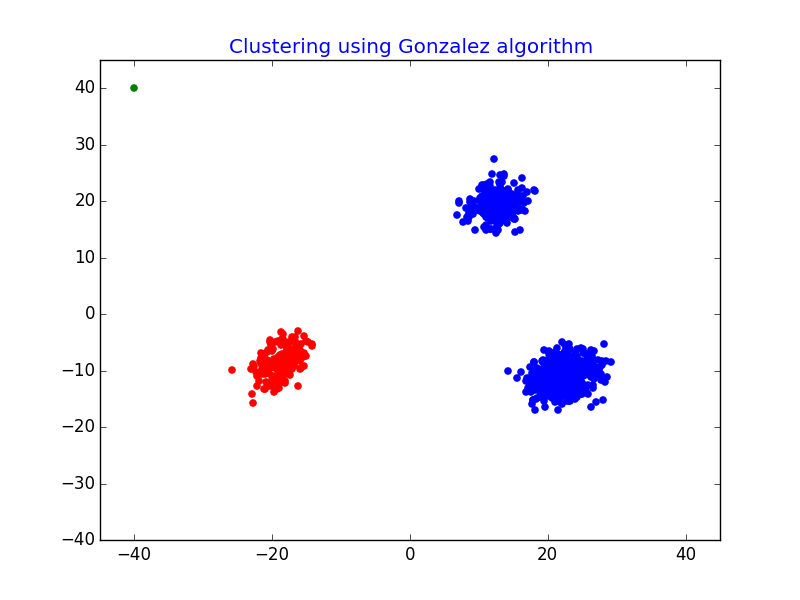
\includegraphics[width=5cm]{Gonzalez} }}%
	\end{figure}

From the plot we can clearly observe that the point (-40,40) on the top left is an outlier and since Gonzalez algorithm biases towards outliers it picks that point as one of the cluster centers. Since all the other points are at farther distance from that point, we have only that point in one of the clusters. The remaining points are then assigned to the other two cluster centers.

\item[] \underline{\textbf{\emph k-Means++ Algorithm}}

In k-Means++ algorithm we start out by choosing $c_1$ as the point with index 1. We then determine the next $c_i$ value by picking an element with a probability ptoportional to the $(Distance) ^2 $. We basically fit in the values we get into a distribution and then randomly pick a center from the distribution. Once we obtain the center we then update the points to the new centers if they are closer to the new center then the previous centers and then repeat the whole process until we end up with \emph k clusters. In our case \emph k is 3. \\

Since the algorithm is randomized the centers which we obtain changes during every run. However since we always choose the point with index 1 in dataset C2.txt as $c_1$ our $c_1$ would always be the same. It would be $c_2$ and $c_3$ which would vary in our case.

I ran 20 different trails for the k-Means++ algorithm and wrote the centers and the 3-means cost into a text file. 3-means cost was computed using the following expression:

\begin{center}
	$\sum_{x \in X}^{} (\textbf{d}(x,\phi_c(x) ))^2$
\end{center} 

I then plotted the cumulative density function of the 3-means cost and the result is shown below:

	\begin{figure}[H]%
		\centering
		\subfloat[ Point Assignment Clustering- k-Means++ Algorithm]{{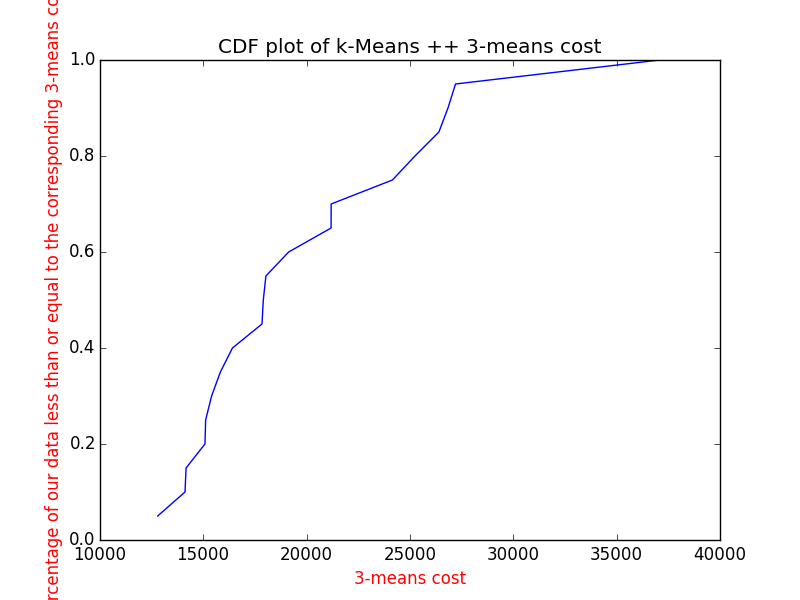
\includegraphics[width=6cm]{CDF_2aa} }}%
	\end{figure}

Thus we can see that more than 60\% of the values of our cost function are lesser than 25000.

I plotted the output of few trials and found that k-means++ never picked the outlier point as one of its centers. The probability of k-Means ++ picking the outlier point is very low. Hence it does a slightly better job of picking the centers than compared to Gonzalez but the computation is slightly more involved when compared to Gonzalez.

Because of the above mentioned reason when I ran for 20 trials, \textbf{ there were zero times} when the fraction of subsets from the k-Means++ was same as that of Gonzalez algoirthm. But if we maybe run say 1000 trials then there might be a possible opportunity that k-means ++ might pick (-40,40) as one of its centers. 


\item[] \textbf{ Part B}

\item[] \underline{\textbf{Lloyd's Algorithm}}

In this part we experiment with the Lloyd's algorithm for \emph k-means clustering. In Lloyds algorithm we initally choose a set of k centers randomly and then perform the averaging operation to get a better cluster center. In our problem instead of having to randomly choose the centers we have been provided with the initial centers.

\textbf{ Lloyds algorithm with C initially with points indexed {1,2,3} }\\
\begin{itemize}
	\item[] \textbf{Final Centers}: \{(-19.081733907108436, -8.281661740626506), (22.133750014182453, -10.901101209623068), (12.629664864101152, 19.363135342451358)\}
	
	\item[] \textbf{3-means cost}: 12683.2923315
	\item[] \textbf{No of points having center as $c_1$}: 166 
	\item[] \textbf{No of points having center as $c_2$}: 581 
	\item[] \textbf{No of points having center as $c_3$}: 257 
\end{itemize}

\textbf{Subsets}:

\textbf{Indexes of the points which have their center as  (-19.081733907108436, -8.281661740626506)}

[1, 4, 5, 6, 7, 8, 9, 10, 11, 12, 13, 14, 15, 16, 17, 18, 19, 20, 21, 22, 23, 24, 25, 26, 27, 28, 29, 30, 31, 32, 33, 34, 35, 36, 37, 38, 39, 40, 41, 42, 43, 44, 45, 46, 47, 48, 49, 50, 51, 52, 53, 54, 55, 56, 57, 58, 59, 60, 61, 62, 63, 64, 65, 66, 67, 68, 69, 70, 71, 72, 73, 74, 75, 76, 77, 78, 79, 80, 81, 82, 83, 84, 85, 86, 87, 88, 89, 90, 91, 92, 93, 94, 95, 96, 97, 98, 99, 100, 101, 102, 103, 104, 105, 106, 107, 108, 109, 110, 111, 112, 113, 114, 115, 116, 117, 118, 119, 120, 121, 122, 123, 124, 125, 126, 127, 128, 129, 130, 131, 132, 133, 134, 135, 136, 137, 138, 139, 140, 141, 142, 143, 144, 145, 146, 147, 148, 149, 150, 151, 152, 153, 154, 155, 156, 157, 158, 159, 160, 161, 162, 163, 164, 165, 166, 167, 1004]

\textbf{Indexes of the points which have their center as  (22.133750014182453, -10.901101209623068)}

[2, 168, 169, 170, 171, 172, 173, 174, 175, 176, 177, 178, 179, 180, 181, 182, 183, 184, 185, 186, 187, 188, 189, 190, 191, 192, 193, 194, 195, 196, 197, 198, 199, 200, 201, 202, 203, 204, 205, 206, 207, 208, 209, 210, 211, 212, 213, 214, 215, 216, 217, 218, 219, 220, 221, 222, 223, 224, 225, 226, 227, 228, 229, 230, 231, 232, 233, 234, 235, 236, 237, 238, 239, 240, 241, 242, 243, 244, 245, 246, 247, 248, 249, 250, 251, 252, 253, 254, 255, 256, 257, 258, 259, 260, 261, 262, 263, 264, 265, 266, 267, 268, 269, 270, 271, 272, 273, 274, 275, 276, 277, 278, 279, 280, 281, 282, 283, 284, 285, 286, 287, 288, 289, 290, 291, 292, 293, 294, 295, 296, 297, 298, 299, 300, 301, 302, 303, 304, 305, 306, 307, 308, 309, 310, 311, 312, 313, 314, 315, 316, 317, 318, 319, 320, 321, 322, 323, 324, 325, 326, 327, 328, 329, 330, 331, 332, 333, 334, 335, 336, 337, 338, 339, 340, 341, 342, 343, 344, 345, 346, 347, 348, 349, 350, 351, 352, 353, 354, 355, 356, 357, 358, 359, 360, 361, 362, 363, 364, 365, 366, 367, 368, 369, 370, 371, 372, 373, 374, 375, 376, 377, 378, 379, 380, 381, 382, 383, 384, 385, 386, 387, 388, 389, 390, 391, 392, 393, 394, 395, 396, 397, 398, 399, 400, 401, 402, 403, 404, 405, 406, 407, 408, 409, 410, 411, 412, 413, 414, 415, 416, 417, 418, 419, 420, 421, 422, 423, 424, 425, 426, 427, 428, 429, 430, 431, 432, 433, 434, 435, 436, 437, 438, 439, 440, 441, 442, 443, 444, 445, 446, 447, 448, 449, 450, 451, 452, 453, 454, 455, 456, 457, 458, 459, 460, 461, 462, 463, 464, 465, 466, 467, 468, 469, 470, 471, 472, 473, 474, 475, 476, 477, 478, 479, 480, 481, 482, 483, 484, 485, 486, 487, 488, 489, 490, 491, 492, 493, 494, 495, 496, 497, 498, 499, 500, 501, 502, 503, 504, 505, 506, 507, 508, 509, 510, 511, 512, 513, 514, 515, 516, 517, 518, 519, 520, 521, 522, 523, 524, 525, 526, 527, 528, 529, 530, 531, 532, 533, 534, 535, 536, 537, 538, 539, 540, 541, 542, 543, 544, 545, 546, 547, 548, 549, 550, 551, 552, 553, 554, 555, 556, 557, 558, 559, 560, 561, 562, 563, 564, 565, 566, 567, 568, 569, 570, 571, 572, 573, 574, 575, 576, 577, 578, 579, 580, 581, 582, 583, 584, 585, 586, 587, 588, 589, 590, 591, 592, 593, 594, 595, 596, 597, 598, 599, 600, 601, 602, 603, 604, 605, 606, 607, 608, 609, 610, 611, 612, 613, 614, 615, 616, 617, 618, 619, 620, 621, 622, 623, 624, 625, 626, 627, 628, 629, 630, 631, 632, 633, 634, 635, 636, 637, 638, 639, 640, 641, 642, 643, 644, 645, 646, 647, 648, 649, 650, 651, 652, 653, 654, 655, 656, 657, 658, 659, 660, 661, 662, 663, 664, 665, 666, 667, 668, 669, 670, 671, 672, 673, 674, 675, 676, 677, 678, 679, 680, 681, 682, 683, 684, 685, 686, 687, 688, 689, 690, 691, 692, 693, 694, 695, 696, 697, 698, 699, 700, 701, 702, 703, 704, 705, 706, 707, 708, 709, 710, 711, 712, 713, 714, 715, 716, 717, 718, 719, 720, 721, 722, 723, 724, 725, 726, 727, 728, 729, 730, 731, 732, 733, 734, 735, 736, 737, 738, 739, 740, 741, 742, 743, 744, 745, 746, 747]

\textbf{Indexes of the points which have their center as  (12.629664864101152, 19.363135342451358)}

[3, 748, 749, 750, 751, 752, 753, 754, 755, 756, 757, 758, 759, 760, 761, 762, 763, 764, 765, 766, 767, 768, 769, 770, 771, 772, 773, 774, 775, 776, 777, 778, 779, 780, 781, 782, 783, 784, 785, 786, 787, 788, 789, 790, 791, 792, 793, 794, 795, 796, 797, 798, 799, 800, 801, 802, 803, 804, 805, 806, 807, 808, 809, 810, 811, 812, 813, 814, 815, 816, 817, 818, 819, 820, 821, 822, 823, 824, 825, 826, 827, 828, 829, 830, 831, 832, 833, 834, 835, 836, 837, 838, 839, 840, 841, 842, 843, 844, 845, 846, 847, 848, 849, 850, 851, 852, 853, 854, 855, 856, 857, 858, 859, 860, 861, 862, 863, 864, 865, 866, 867, 868, 869, 870, 871, 872, 873, 874, 875, 876, 877, 878, 879, 880, 881, 882, 883, 884, 885, 886, 887, 888, 889, 890, 891, 892, 893, 894, 895, 896, 897, 898, 899, 900, 901, 902, 903, 904, 905, 906, 907, 908, 909, 910, 911, 912, 913, 914, 915, 916, 917, 918, 919, 920, 921, 922, 923, 924, 925, 926, 927, 928, 929, 930, 931, 932, 933, 934, 935, 936, 937, 938, 939, 940, 941, 942, 943, 944, 945, 946, 947, 948, 949, 950, 951, 952, 953, 954, 955, 956, 957, 958, 959, 960, 961, 962, 963, 964, 965, 966, 967, 968, 969, 970, 971, 972, 973, 974, 975, 976, 977, 978, 979, 980, 981, 982, 983, 984, 985, 986, 987, 988, 989, 990, 991, 992, 993, 994, 995, 996, 997, 998, 999, 1000, 1001, 1002, 1003]


I also plotted the data to verify if the results were making sense. The results are shown below:

\begin{figure}[H]%
	\centering
	\qquad
	\subfloat[Lloyd's algorithm]{{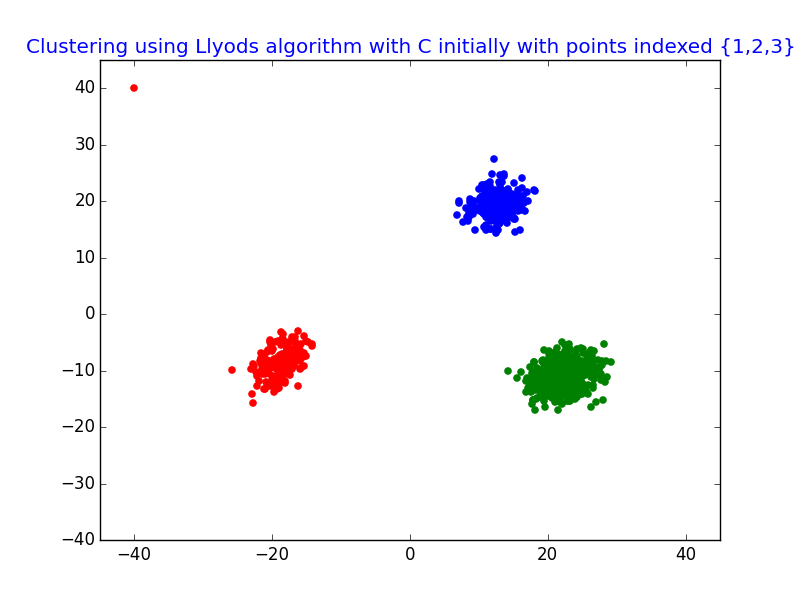
\includegraphics[width=5cm]{Lloyds_a} }}%
\end{figure}	

We can see that the Lloyd's algorithm performs a very good job of finding the cluster centers and also makes sure the outlier points isn't taken with the same weight as a data point. Thus we get three discernible clusters.


\textbf{ Lloyds algorithm with C initially as the output of Gonzalez algorithm }\\
\begin{itemize}
	\item[] \textbf{Final Centers}: \{ (-18.95495653684849, -8.574277872387878), (-40.0, 40.0), (19.219012682952254, -1.6195871357768579)    \}
    	\item[] \textbf{3-means cost}: 189194.33209
    	\item[] \textbf{No of points having center as $c_1$}: 165
    	\item[] \textbf{No of points having center as $c_2$}: 1 
    	\item[] \textbf{No of points having center as $c_3$}: 838
    	\end{itemize}
    	
    	\textbf{Subsets:}
    	
    	\textbf{Indexes of the points which have their center as  -18.95495653684849, -8.574277872387878)}
    	
    	[1, 4, 5, 6, 7, 8, 9, 10, 11, 12, 13, 14, 15, 16, 17, 18, 19, 20, 21, 22, 23, 24, 25, 26, 27, 28, 29, 30, 31, 32, 33, 34, 35, 36, 37, 38, 39, 40, 41, 42, 43, 44, 45, 46, 47, 48, 49, 50, 51, 52, 53, 54, 55, 56, 57, 58, 59, 60, 61, 62, 63, 64, 65, 66, 67, 68, 69, 70, 71, 72, 73, 74, 75, 76, 77, 78, 79, 80, 81, 82, 83, 84, 85, 86, 87, 88, 89, 90, 91, 92, 93, 94, 95, 96, 97, 98, 99, 100, 101, 102, 103, 104, 105, 106, 107, 108, 109, 110, 111, 112, 113, 114, 115, 116, 117, 118, 119, 120, 121, 122, 123, 124, 125, 126, 127, 128, 129, 130, 131, 132, 133, 134, 135, 136, 137, 138, 139, 140, 141, 142, 143, 144, 145, 146, 147, 148, 149, 150, 151, 152, 153, 154, 155, 156, 157, 158, 159, 160, 161, 162, 163, 164, 165, 166, 167]
    	
    	\textbf{Indexes of the points which have their center as  (-40,40)}
    	
    	 [1004]
    	 
    	 \textbf{Indexes of the points which have their center as  (19.219012682952254, -1.6195871357768579) }
    	 
    	 [2, 3, 168, 169, 170, 171, 172, 173, 174, 175, 176, 177, 178, 179, 180, 181, 182, 183, 184, 185, 186, 187, 188, 189, 190, 191, 192, 193, 194, 195, 196, 197, 198, 199, 200, 201, 202, 203, 204, 205, 206, 207, 208, 209, 210, 211, 212, 213, 214, 215, 216, 217, 218, 219, 220, 221, 222, 223, 224, 225, 226, 227, 228, 229, 230, 231, 232, 233, 234, 235, 236, 237, 238, 239, 240, 241, 242, 243, 244, 245, 246, 247, 248, 249, 250, 251, 252, 253, 254, 255, 256, 257, 258, 259, 260, 261, 262, 263, 264, 265, 266, 267, 268, 269, 270, 271, 272, 273, 274, 275, 276, 277, 278, 279, 280, 281, 282, 283, 284, 285, 286, 287, 288, 289, 290, 291, 292, 293, 294, 295, 296, 297, 298, 299, 300, 301, 302, 303, 304, 305, 306, 307, 308, 309, 310, 311, 312, 313, 314, 315, 316, 317, 318, 319, 320, 321, 322, 323, 324, 325, 326, 327, 328, 329, 330, 331, 332, 333, 334, 335, 336, 337, 338, 339, 340, 341, 342, 343, 344, 345, 346, 347, 348, 349, 350, 351, 352, 353, 354, 355, 356, 357, 358, 359, 360, 361, 362, 363, 364, 365, 366, 367, 368, 369, 370, 371, 372, 373, 374, 375, 376, 377, 378, 379, 380, 381, 382, 383, 384, 385, 386, 387, 388, 389, 390, 391, 392, 393, 394, 395, 396, 397, 398, 399, 400, 401, 402, 403, 404, 405, 406, 407, 408, 409, 410, 411, 412, 413, 414, 415, 416, 417, 418, 419, 420, 421, 422, 423, 424, 425, 426, 427, 428, 429, 430, 431, 432, 433, 434, 435, 436, 437, 438, 439, 440, 441, 442, 443, 444, 445, 446, 447, 448, 449, 450, 451, 452, 453, 454, 455, 456, 457, 458, 459, 460, 461, 462, 463, 464, 465, 466, 467, 468, 469, 470, 471, 472, 473, 474, 475, 476, 477, 478, 479, 480, 481, 482, 483, 484, 485, 486, 487, 488, 489, 490, 491, 492, 493, 494, 495, 496, 497, 498, 499, 500, 501, 502, 503, 504, 505, 506, 507, 508, 509, 510, 511, 512, 513, 514, 515, 516, 517, 518, 519, 520, 521, 522, 523, 524, 525, 526, 527, 528, 529, 530, 531, 532, 533, 534, 535, 536, 537, 538, 539, 540, 541, 542, 543, 544, 545, 546, 547, 548, 549, 550, 551, 552, 553, 554, 555, 556, 557, 558, 559, 560, 561, 562, 563, 564, 565, 566, 567, 568, 569, 570, 571, 572, 573, 574, 575, 576, 577, 578, 579, 580, 581, 582, 583, 584, 585, 586, 587, 588, 589, 590, 591, 592, 593, 594, 595, 596, 597, 598, 599, 600, 601, 602, 603, 604, 605, 606, 607, 608, 609, 610, 611, 612, 613, 614, 615, 616, 617, 618, 619, 620, 621, 622, 623, 624, 625, 626, 627, 628, 629, 630, 631, 632, 633, 634, 635, 636, 637, 638, 639, 640, 641, 642, 643, 644, 645, 646, 647, 648, 649, 650, 651, 652, 653, 654, 655, 656, 657, 658, 659, 660, 661, 662, 663, 664, 665, 666, 667, 668, 669, 670, 671, 672, 673, 674, 675, 676, 677, 678, 679, 680, 681, 682, 683, 684, 685, 686, 687, 688, 689, 690, 691, 692, 693, 694, 695, 696, 697, 698, 699, 700, 701, 702, 703, 704, 705, 706, 707, 708, 709, 710, 711, 712, 713, 714, 715, 716, 717, 718, 719, 720, 721, 722, 723, 724, 725, 726, 727, 728, 729, 730, 731, 732, 733, 734, 735, 736, 737, 738, 739, 740, 741, 742, 743, 744, 745, 746, 747, 748, 749, 750, 751, 752, 753, 754, 755, 756, 757, 758, 759, 760, 761, 762, 763, 764, 765, 766, 767, 768, 769, 770, 771, 772, 773, 774, 775, 776, 777, 778, 779, 780, 781, 782, 783, 784, 785, 786, 787, 788, 789, 790, 791, 792, 793, 794, 795, 796, 797, 798, 799, 800, 801, 802, 803, 804, 805, 806, 807, 808, 809, 810, 811, 812, 813, 814, 815, 816, 817, 818, 819, 820, 821, 822, 823, 824, 825, 826, 827, 828, 829, 830, 831, 832, 833, 834, 835, 836, 837, 838, 839, 840, 841, 842, 843, 844, 845, 846, 847, 848, 849, 850, 851, 852, 853, 854, 855, 856, 857, 858, 859, 860, 861, 862, 863, 864, 865, 866, 867, 868, 869, 870, 871, 872, 873, 874, 875, 876, 877, 878, 879, 880, 881, 882, 883, 884, 885, 886, 887, 888, 889, 890, 891, 892, 893, 894, 895, 896, 897, 898, 899, 900, 901, 902, 903, 904, 905, 906, 907, 908, 909, 910, 911, 912, 913, 914, 915, 916, 917, 918, 919, 920, 921, 922, 923, 924, 925, 926, 927, 928, 929, 930, 931, 932, 933, 934, 935, 936, 937, 938, 939, 940, 941, 942, 943, 944, 945, 946, 947, 948, 949, 950, 951, 952, 953, 954, 955, 956, 957, 958, 959, 960, 961, 962, 963, 964, 965, 966, 967, 968, 969, 970, 971, 972, 973, 974, 975, 976, 977, 978, 979, 980, 981, 982, 983, 984, 985, 986, 987, 988, 989, 990, 991, 992, 993, 994, 995, 996, 997, 998, 999, 1000, 1001, 1002, 1003]
    	 
    	
    	
    	I also plotted the data to verify if the results were making sense. The results are shown below:
    	
    	\begin{figure}[H]%
    		\centering
    		\qquad
    		\subfloat[Lloyd's algorithm]{{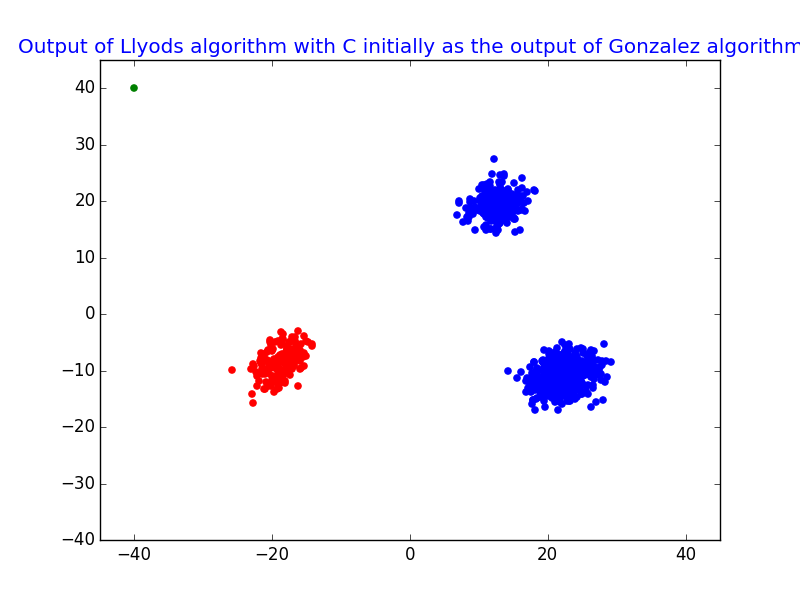
\includegraphics[width=5cm]{Lloyds_b} }}%
    	\end{figure}	
    	

\textbf{ Lloyds algorithm with C initially as output of k-Means ++ }\\
Here we use the ouput of the different runs of k-Means++ in the previous part as the initial centers for our lloyd's alogorithm. Since the centers are different every single time, we plot the cdf  of the 3-means cost.

The results are shown below:

\begin{figure}[H]%
	\centering
	\qquad
	\subfloat[Lloyd's algorithm using k-means++ input]{{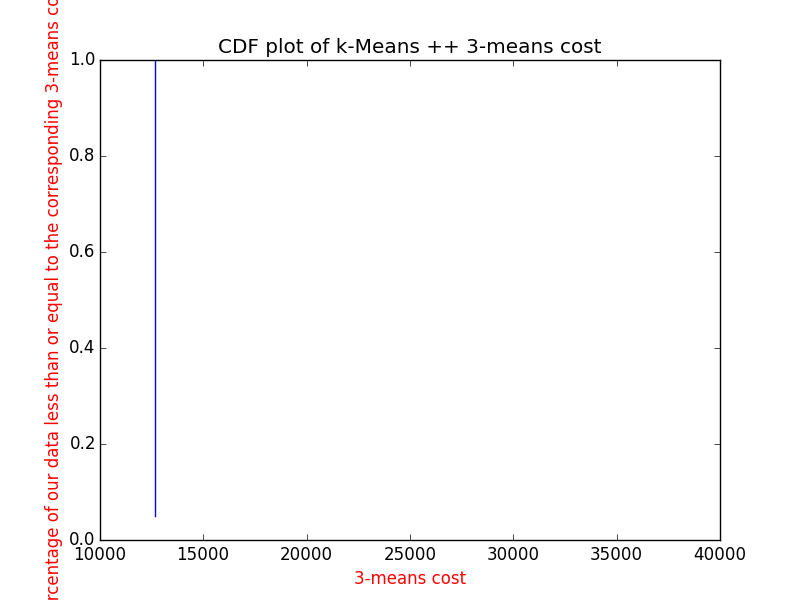
\includegraphics[width=5cm]{CDF_2b} }}%
\end{figure}	

I observed that LLoyds algorithm was giving the same set of centers for the different inputs provided by K-means ++. This goes to show that Lloyds algorithm does a very good job when its inital centers are being provided by the K-means ++ . Also the K-means++ algorithm is good enough to be given as the input to this algorithm and performs better when done so. The CDF clearly shows that the straight line corresponds to one single cost namely \textbf{12683.2923315}. The Lloyds algorithm performs very good averaging.

The output produced by the Lloyds algorithm in these cases are shown below:

\begin{figure}[H]%
	\centering
	\qquad
	\subfloat[Lloyd's algorithm using k-means++ input]{{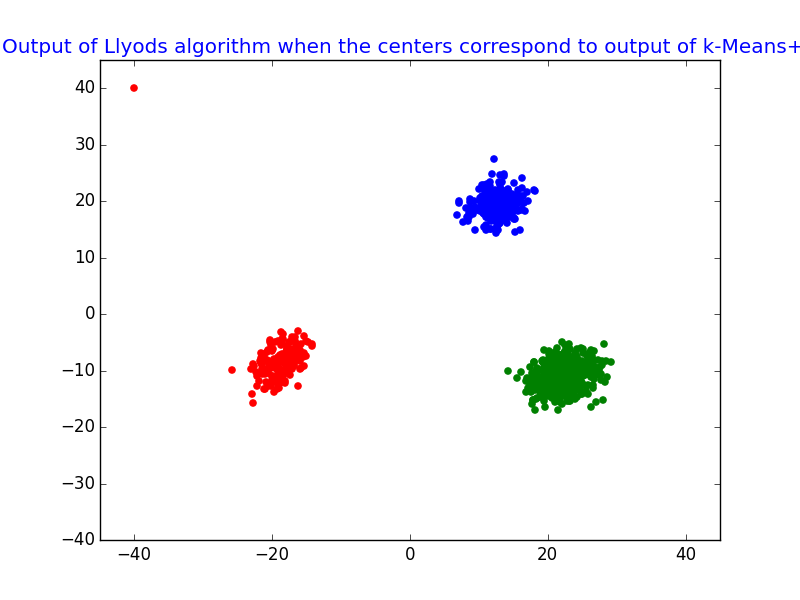
\includegraphics[width=5cm]{Lloydsc_1} }}%
	\qquad
	\subfloat[Lloyd's algorithm using k-means++ input]{{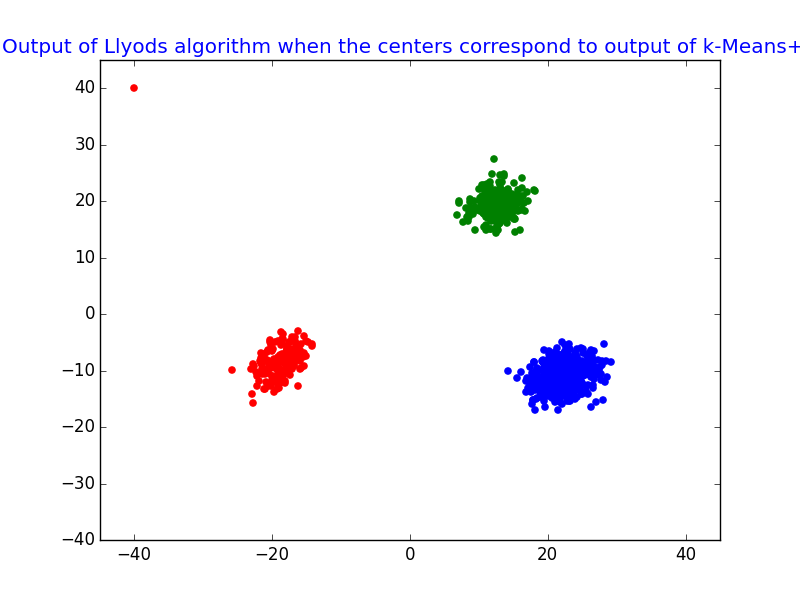
\includegraphics[width=5cm]{Lloydsc_2} }}%
\end{figure}	

We can	clearly see that it produces discernible clusters.

Also like in the previous case, \textbf{ there were 0 trials } during which the subsets produced by the Lloyds algorithm were same as that of the input. Again these were for the 20 trials which I had made. Since Lloyd's algorithm always tries to push the center towards the middle, there were always differences in the subsets produced by the Lloyd and the input from k-Means++.


\textbf{Part C}

In order to prove the given result, I have approached the problem based on the steps provided in the question.

\begin{itemize}
	\item \textbf{ Proving the results for $S \in R ^1$}
	
	If we consider one dimension then everything could be considered as points. Sum of the squared distance between a point and its center would actually be the average of all the points which is nothing but the expression provided on the right hand side.Hence this is true for one dimension
	
	\item Expanding each term we get $(d(x,p))^2 =(x-p)^2 =x^2 +p^2 -2*x*p$
	
	When we take the first derivative with respect to x, we get :\\
	2x -2p \\
	
	When we take summation of the above expression we end up with \\
	$ 2 \cdot \sum_{x \in S}^{} x  -2p \sum_{}^{} 1 $\\
	p is constant term and summation over 1 is also constant.
	
	Hence we are left with  $2\sum_{x \in S}^{} x $\\
	
	In a right angled triangle the length of the hypotenuse will always be greater than any of the other two sides but also it maintains another property of traingle where in the sum of two sides is greater than the greatest side. Therfore the distance will always be equal to the mean of the points i.e sum of all the points divided by the total number of points. This is what the RHS of the expression is.
	
	Hence this could be considered as the proof.
	
\end{itemize}

	
 \end{itemize}
 

\section{k-Median Clustering}

\begin{itemize}
	\item[] \textbf{Part A}
	
	\underline{\textbf{4-median problem} }\\
	
	In this part of the question we implement the k-Median clustering formulation. For this question we make use of the dataset C3.txt and we are asked to find a set of 4 centers $C={c_1,c_2,c_3,c_4}$
	
	\textbf{ Logic implemented:}
	\begin{itemize}
		\item Initalize the 4 centers randomly with 4 points from the data set.
		\item Map each point in the dataset to its closest center.This will give us a set of clusters one for each center.
		\item For each cluster which we obtained, compute the 1-median. find the 1-median.This is that point in the cluster for which the sum of the distances to the remaining points in the cluster is as small as possible. 
		\item At the same time keep track of the cost function. Cost is given by $Cost_1(P,C)= \sum_{p \in P}^{}\textbf{d}(p,\phi_c(p)))$. When the difference in the cost function between two successive iterations is less than 1, stop and report the centers.
	\end{itemize}
	
	I implemented it similar to Lloyds algorithm. The terminating condition for thw while loop will be the fact that cost function difference between successive iterations is  less than 1.
	
	After having implemented the algorithm and ran it for several trials, the minimum cost that I could obtain was \textbf{4889.54714005} and the centers corresponding to this cost function are given below:
	
	\textbf{ Centers}
	\begin{itemize}
		\item \textbf{C1}= ( 7.304007052	2.715665123	0.272342366	-0.8475510012	-0.7436087533) 
		\item \textbf{C2} =(0.2192894743	0.5102981586	0.3356793955	10.1052917	0.007539507597)
		\item \textbf{C3} = (0.05613336132	-0.1974222365	10.62588277	0.4938042239	0.0275396858)
		\item \textbf{C4} = (0.08501570631	-0.1444334263	0.001343366922	-0.03196316278	10.19040183)
		
	\end{itemize}
	
	
\item[] \textbf{Part B}

\underline{\textbf{5-medians}}

In this part of the question we are expected to run our algorithm for the 5-medians problem. Interestingly for 5-median clustering problem the minimum cost function value that was obtained by my program was \textbf{3015.74701234}\\

The set of centers corresponding to this cost function value are given below:

	\textbf{ Centers}
	\begin{itemize}
		\item \textbf{C1}= ( 0.08501570631	-0.1444334263	0.001343366922	-0.03196316278	10.19040183) 
		\item \textbf{C2} =(0.3770908042	10.17701081	0.01742525472	0.4741579895	-0.211318625)
		\item \textbf{C3} = (0.05613336132	-0.1974222365	10.62588277	0.4938042239	0.02753968588)
		\item \textbf{C4} = (9.22103491	0.1824501818	-0.6434791183	-0.2129211518	-0.6665713908
		)
		\item \textbf{C5}=(0.2192894743	0.5102981586	0.3356793955	10.1052917	0.007539507597
		)
	\end{itemize}
	
On observation 3 of the 5 centers seem to match exactly with the lowest cost function value for the 4-median clustering. And one more interesting feature which I observed in 5-median clustering was with the centers specified, all the clusters had an equal number of points which were 200 in total.	
 
\end{itemize}


\end{document}
